\documentclass[12pt]{article}
\usepackage{geometry}
\usepackage{dcolumn}
\usepackage{booktabs}
\usepackage{pdflscape}
\usepackage{graphicx}
\usepackage{placeins}
\usepackage{dcolumn}
\usepackage{xcolor}
\usepackage{booktabs}
\linespread{1.5}
\usepackage{subcaption}
\usepackage{amsmath}
\usepackage{hyperref}
\usepackage{multirow}
\usepackage[title]{appendix}
\usepackage{xepersian}
\settextfont{XB Zar}
\setdigitfont{XB Zar}

\begin{document}
\title{سهام مرتبط}
\author{سید مرتضی آقاجان‌زاده}
\maketitle

در بازار بورس اوراق بهادار تهران ساختار سهام‌داری و مالکیتی درهم‌تنیده‌ای شکل‌گرفته است. به صورتی که یک نماد بورسی می‌تواند دارای ده‌ها مالک بورسی و غیر بورسی باشد. از سهام دارای سهام‌دار مشترک، به سهام مرتبط
\LTRfootnote{\lr{ Connected Stocks}}
 تعبیر می‌شود. سؤال اصلی این است که آیا با کنترل ویژگی‌های دو نماد و شباهت‌های میان بخشی، با افزایش درجه‌ی سهام‌داری مشترک، رفتار قیمتی دو نماد تغیر می‌کند؟ 

به دلیل ضعف زیرساخت‌های قانونی در این بازار، سهام‌داران عمده با حفظ منافع شخصی خود جهت استفاده از منافع سهام‌داران خرد به تشکیل ساختارهای هرمی 
\LTRfootnote{\lr{Pyramidal ownership}}
و ضربدری 
\LTRfootnote{\lr{Cross ownership}}
روی می‌آورند تا بدین‌وسیله  حق رأی خود را نسبت به درصد مالکیت افزایش دهند. سهام‌داران عمده معمولاً از مزیت اطلاعاتی نسبت به سهام‌داران خرد برخوردارند.
این عدم تقارن اطلاعات و دسترسی بیشتر به اطلاعات شرکت سبب می‌شود تا سهام‌دار عمده در زمان رونق کسب‌وکار با ممانعت از افشای اطلاعات، سود بیشتری از حق رای خود کسب کند. در مقابل، زمانی که کسب‌وکار دچار ضرر یا رکود شود، سهام‌دار کنترلی با انتشار اطلاعات می‌تواند دیگران را در این زیان شریک کند.


عدم افشای اطلاعات مخصوص شرکت و درنتیجه عدم انعکاس آن در قیمت سهام به این معناست که بخش عظیمی از اطلاعات انعکاس یافته در قیمت و درنتیجه نوسان‌های بازده، از اطلاعات سامان‌مند ناشی می‌شود که این امر سبب می‌شود حرکت هم‌جهت قیمت‌ها، یا به‌اصطلاح هم‌زمانی بازده، افزایش یابد. این سازوکار بر عدم شفافیت اطلاعات شرکت‌ها و درنتیجه عدم انعکاس اطلاعات مخصوص شرکت در قیمت سهام مبتنی است. از طرفی با توجه به حضور سهام‌داران در مجامع عمومی، این سهام‌داران در اتخاذ تصمیمات کلیدی شرکت تأثیرگذار می‌باشند و می‌توانند در حرکت هم‌جهت در نماد‌ها تأثیرگذار باشند.




\section{مطالعات گذشته}
\subsection{\lr{JF-2014-Anton Polk - Connected Stocks}}
\label{s1.1}


این مقاله رفتار نمادهای حاضر در سبد سرمایه‌گذاری صندوق‌های سرمایه‌گذاری مشترک 
\LTRfootnote{\lr{Mutual Funds}}
را مورد بررسی قرار می‌دهد. در این مقاله جهت بررسی درجه اشتراک مالکیت میان دو نماد از نسبت مجموع ارزش  مالکیت مشترک میان دو نماد به کل ارزش بازاری دو نماد استفاده می‌شود و در ادامه با نماد
 $ FCAP_{ij,t} $ 
نشان داده می‌شود. به‌عبارت‌دیگر این متغیر برابر است با:
\begin{equation}
 FCAP_{ij,t} = \frac{\sum_{f = 1}^{F} (S^f_{i,t}P_{i,t}+S^f_{j,t}P_{j,t})}{S_{i,t}P{i,t} + S_{j,t}P{j,t}} 
 \label{e2}
\end{equation}
 که 
 $ S^f_{i,t} $
 بیانگر مالیکت سهام i در زمان t توسط صندوق f و
  $ P_{i,t}$
  قیمت همان سهام در زمان t می‌باشد. 
  منظور از مالکیت مشترک در لحظه t ، حضور دو نماد i و j در سبد سرمایه‌گذاری  یک صندوق می‌باشد. به دلیل قابل‌مقایسه بودن این ملاک میان جفت نمادهای متفاوت در هر جفت، این پارامتر ابتدا تبدیل رتبه‌ای
  \LTRfootnote{Rank-transformed}
   شده است و پس از آن نرمال شده است و پارامتر نرمال شده با
 $ FCAPF^*_{ij,t} $ 
نشان‌داده‌شده است. (میانگین به صفر و انحراف معیار به یک تغییریافته است)
  
  در این مقاله از هم‌بستگی میان باقی‌مانده 
  \LTRfootnote{\lr{Residuals}}
  پیش‌بینی بازده روزانه به‌وسیله  مدل چهار عاملی استفاده‌شده است.
   مدل مورد بررسی مقاله در رابطه 
  \ref{e1}
  بیان شده است. در این مدل پارامتر مورد بررسی
 $ b_f $ 
می‌باشد.

  
  \begin{equation}
  \rho_{ij,t+1} = a + b_f \times FCAPF^*_{ij,t} + \sum_{k = 1}^{n } CONTROL_{ij,t,k} + \varepsilon_{ij,t+1}
  \label{e1}
  \end{equation}
  م  دغدغه اصلی نگارنده وجود درون‌زایی‌های ناشی از ملاک‌های انتخاب توسط مدیران صندوق‌های می‌باشد و به‌این‌علت از کنترل‌های متنوعی استفاده می‌کند. در شکل 
    \ref{g1}
     خروجی‌های مدل مقاله ارائه شده است. متغیر 
     $ A_ {ij,t} $
    تعداد تحلیلگران بازار مالی است که برای دو سهم i و j حداقل یک گزارش مالی سالانه منتشر کرده باشند. 
    برای کنترل شباهت دو سهام، یکی از مشخصات شباهت را در هر دوره بر اساس صدک رتبه‌بندی می‌کنیم و پارامتر مورد بررسی از منفی مقدار اختلاف تفاوت صدکی این ملاک شباهت می‌باشد. در مقاله از مشخصات اندازه، B/M و نوسان سهم استفاده شده است.
  
  
  \begin{figure}[htbp]
  \centering
  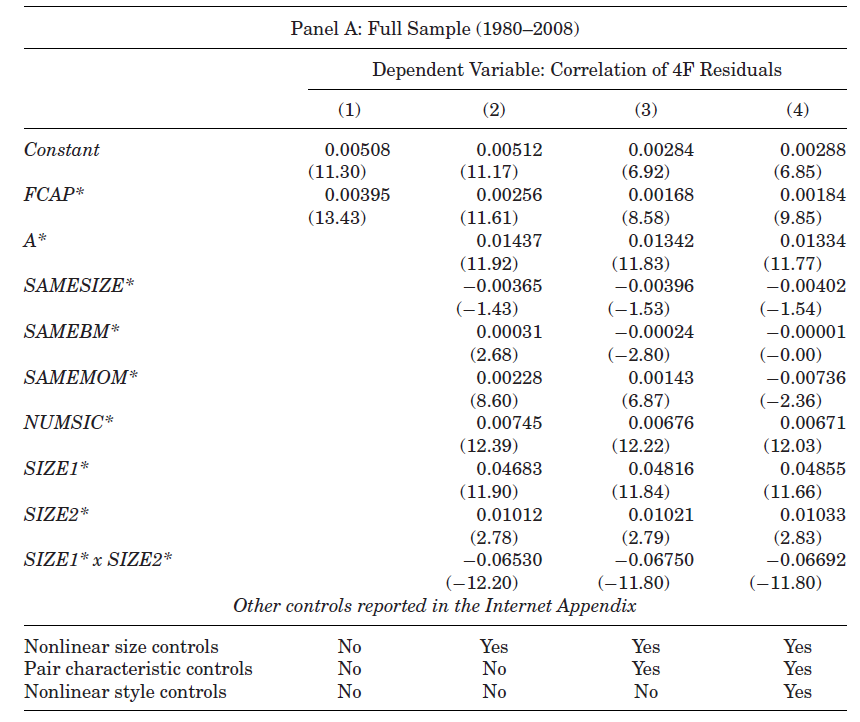
\includegraphics[width=\columnwidth]{Table1.png}
  \caption{ خروجی مدل مقاله \lr{Connected Stocks} }
  \label{g1}
 
  \end{figure}  
\FloatBarrier


\subsection{ساختار بنگاه داری و رفتار بازده سهام: شواهدی از بورس اوراق بهادار تهران}
\label{s1.2}
این پژوهش ابتدا ابعاد و ساختار بنگاه‌داری هرمی و ضربدری در ایران بررسی کرده است. در این راستا از سه تعریف شبکه‌های مدیریتی، سهام‌داری و مالکیتی بهره گرفته شده است؛ در شبکه مدیریتی، در صورت وجود عضو مشترک بین مدیران ارشد شامل اعضای هیئت‌مدیره و مدیرعامل دو شرکت، آن دو را مرتبط در نظر گرفته است. در شبکه سهام‌داری، چنانچه شرکتی سهام‌دار شرکت دیگر باشد و در شبکه مالکیتی به‌واسطه وجود یک سهام‌دار مشترک دو شرکت را مرتبط در نظر گرفته است. در شکل‌های
\ref{m}-\ref{h}
گراف شبکه‌های متفاوت رسم شده است.


\begin{figure}[htbp]
\centering
  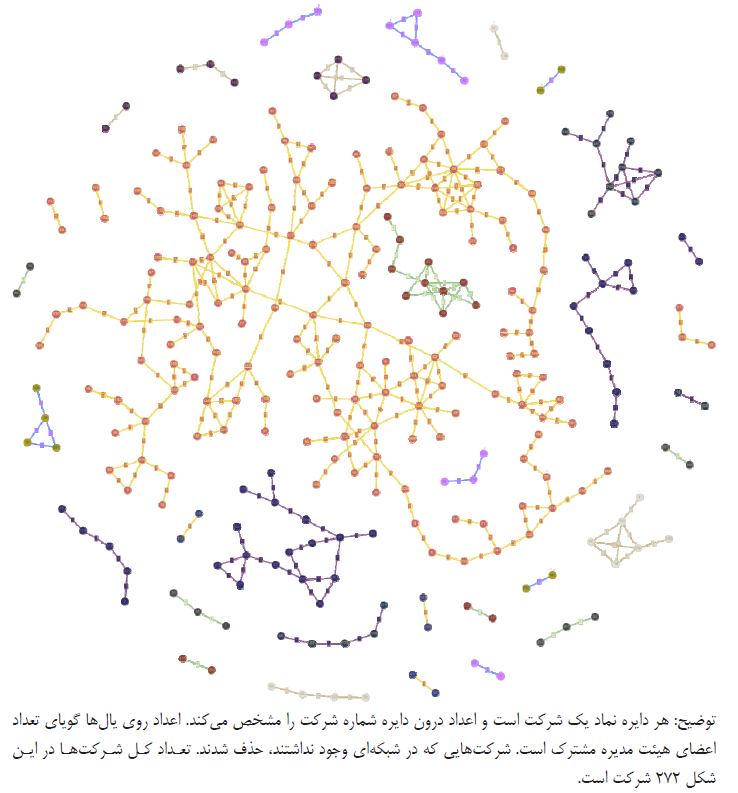
\includegraphics[width=0.6\linewidth]{m.png}
  \caption{گراف شبکه مدیریتی }
  \label{m}
 \end{figure} 
\begin{figure}[htbp]
\centering
  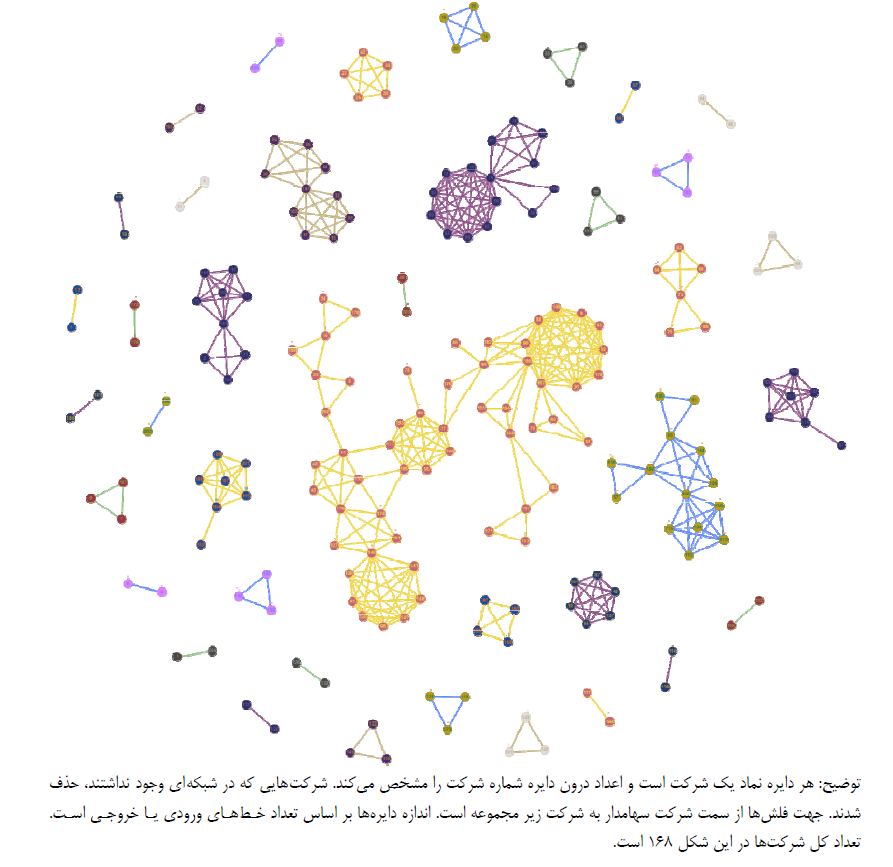
\includegraphics[width=0.6\linewidth]{h1.png}
  \caption{گراف شبکه سهام‌داری برای آستانه 30 درصد }
  \label{h1}
 \end{figure}
 \begin{figure}[htbp]
 \centering
   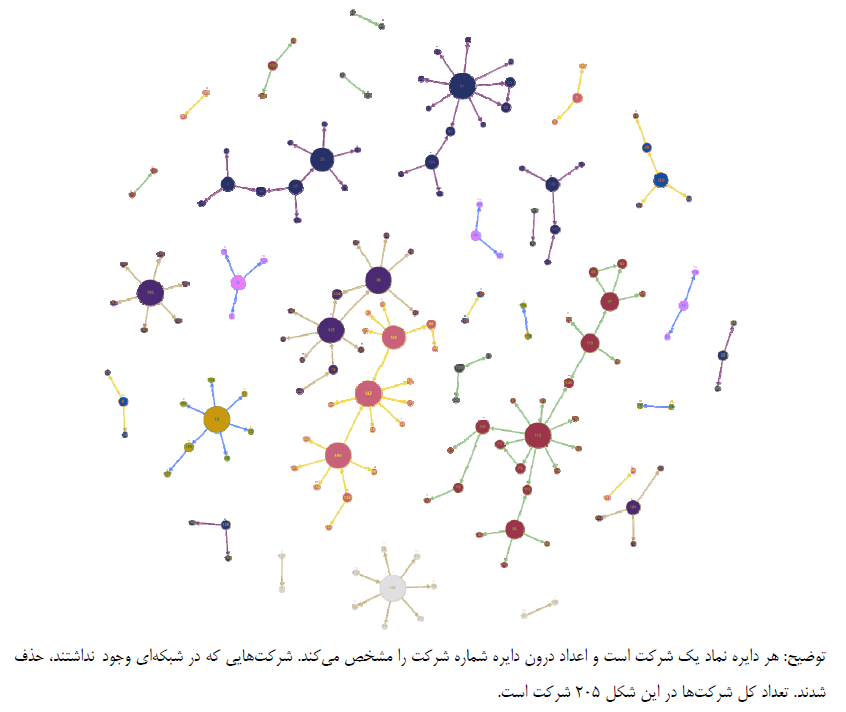
\includegraphics[width=0.6\linewidth]{h.png}
   \caption{گراف شبکه مالکیت برای آستانه 30 درصد }
   \label{h}
  \end{figure}
%\newpage
\FloatBarrier

در ادامه به‌منظور محاسبه هم‌بستگی بازده نمادهای موجود در شبکه‌های تعریف شده از بازده هفتگی سهم استفاده شده است و جهت ازبین‌بردن عوامل برون‌زا از بازده روند زدایی شده استفاده شده است که در روابط زیر تعریف شده است.
\begin{equation}
r_{i,t} = \alpha_i +\beta_i t + \varepsilon_{i,t} \rightarrow r_{i,t} = \hat{\alpha}_i +\hat{\beta}_i t + r^d_{i,t} \Rightarrow r^d_{i,t} = r_{i,t} -\hat{\alpha}_i -\hat{\beta}_i t 
\end{equation}


با توجه به تعریف بازده روند زدایی شده، به‌منظور محاسبه همبستگی دو سهم از دو متغیر وابسته متفاوت استفاده می‌کند. متغیر
 $ f_{i,j} $ 
است که از رابطه شماره
\ref{e3}
بدست می آید و هم حرکتی دو سهم در هفته‌های متفاوت را نشان می‌دهد. دراین‌رابطه، متغیر 
 $ n_{i,j,t}^{up} $ 
چنانچه در هفته $ t $، بازده دو شرکت i و j مثبت باشد برابر با 1 و در غیر این صورت صفر است. به‌صورت مشابه
 $ n_{i,j,t}^{down} $
 برای بازده منفی تعریف شده است.
 $ T_{i,j} $
 تعداد کل هفته‌های مورد بررسی می‌باشد. اگر شاخص هم حرکتی را با بازده‌های روندزدایی شده محاسبه کنیم، آن را شاخص هم حرکتی روندزدایی شده می‌نامد و به‌صورت
 $ f^d_{i,j} $ 
نشان می‌دهد.
\begin{equation}
f_{i,j}  = \frac{\sum_t (n_{i,j,t}^{up}+n_{i,j,t}^{down})}{T_{i,j}}
\label{e3}
\end{equation}

دومین متغیر وابسته مورداستفاده در این پژوهش هم‌بستگی بازده دو سهم می‌باشد که با $ C_{i,j} $ نشان می‌دهد. در تعریف این پارامتر نیز چنانچه از بازده روندزدایی شده استفاده کرده باشد به آن هم‌بستگی روندزدایی شده می‌گوید و با $ C^d_{i,j} $ نشان می‌دهد.

باتوجه‌به تعریف متغیرهای وابسته، متغیر هم حرکتی روندزدایی شده و روندزدایی نشده، هر دو در بازه 
$ [0,1] $
 قرار دارد و متغیر همبستگی روندزدایی شده و روندزدایی نشده نیز در بازه
 $ [-1,1] $
 قرار دارد. باتوجه‌به اینکه مشاهدات نقاط مرزی این پژوهش قابل‌توجه نبوده است از تبدیل لجستیک برای این متغیرها استفاده کرده است. نتایج رگرسیون حداقل مربعات در شکل‌های 
\ref{g2} 
و
\ref{g3}
نشان‌داده‌شده است.

\begin{equation}
\psi_{i,j}^d = \log(\frac{C^d_{i,j}+1}{1-C^d_{i,j}})
\end{equation}

\begin{equation}
\phi_{i,j}^d = \log(\frac{f^d_{i,j}}{1-f^d_{i,j}})
\end{equation}



\begin{landscape}
\begin{figure}
\centering
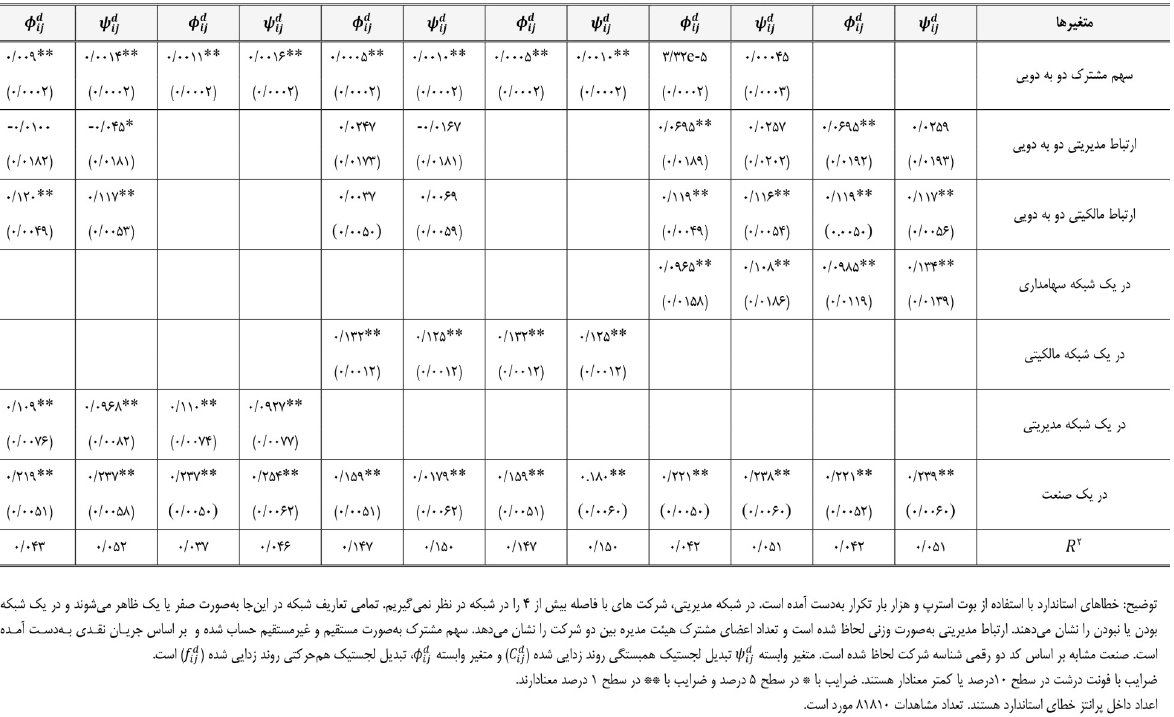
\includegraphics[width=\columnwidth]{Table2.png}
\caption{نتایج رگرسیون حداقل مربعات برای عضویت شرکت‌ها در شبکه‌های مختلف و ارتباط دو به دویی}
\label{g2}
\end{figure}
\begin{figure}
\centering
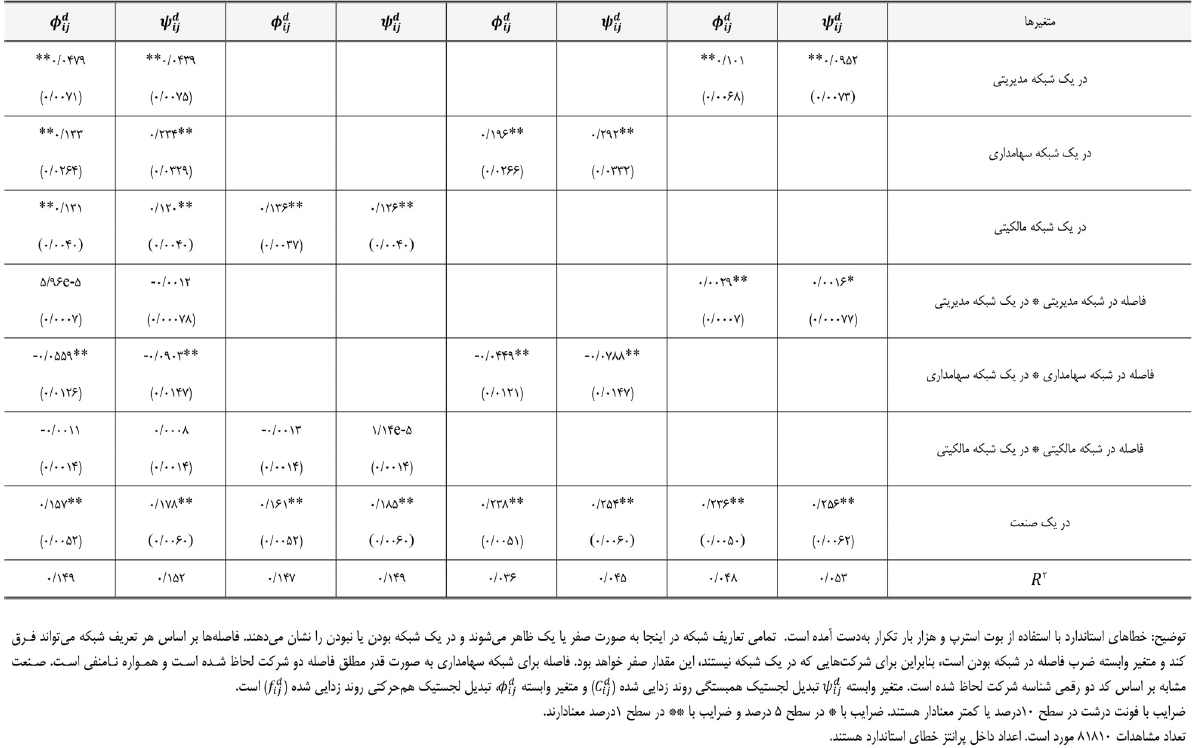
\includegraphics[width=\columnwidth]{Table3.png}
\caption{نتایج رگرسیون حداقل مربعات برای عضویت شرکت‌ها در شبکه‌های مختلف و فاصله آن‌ها در هر شبکه}
\label{g3}
\end{figure}
\end{landscape}


\section{نتایج مقاله با استفاده از داده‌های ایران}
در این قسمت  از داده‌های مالکیت بالای یک درصد سایت 
\lr{TSETMC}
از ابتدای سال 1394 تا تاریخ 1399/08/30 استفاده شده است. در این بازه اطلاعات روزانه سهامداران بالای یک درصد به طور متوسط برای 460 نماد موجود می‌باشد.در این بازه 20817 زوج منحصر به فرد مشاهده شده است که حداقل دارای یک سهام‌دار مشترک بوده‌اند. این مالکیت به صورت متوسط
$ { 398} $
 روز ادامه داشته‌است. در جدول 
\ref{t1}
خلاصه آماری تعداد زوج‌های موجود به صورت روزانه، هفتگی و ماهانه نشان داده‌شده است.

{\begin{table}[htbp]
  \centering
 \lr{ \begin{LTR}
    \begin{tabular}{l|c|cc|ccccc}
        Pairs  & {count} & {mean} &{std} &{min} & 25\%  & 50\%  & 75\%  & {max} \\
          \hline                    
    Daily & 1353  & 6137 & 1050.578 & 2420  & 5300  & 6197  & 7050  & 8108 \\
    Weekly & 350   & 6911 & 1066.878 & 4067  & 6142.75 & 6831.5 & 7894  & 8848 \\
    Monthly & 69    & 7727 & 992.0857 & 4860  & 7037  & 7683  & 8579  & 9269 \\       
    \end{tabular}%}
    \end{LTR}}
      \caption{خلاصه آماری جفت‌های شناسایی شده  }
      \label{t1}
\end{table}}
 \color{black}
 \subsection{محاسبه مالکیت مشترک}
 به منظور محاسبه میزان ارتباط دو نماد در مقاله بخش 
 \ref{s1.1}
  از رابطه  شماره 
 \ref{e2}
 استفاده‌ شده‌است. این ملاک عبارت است  از مجموع ارزش سهام‌داری بخش بر ارزش بازاری نماد که همانطور از تعریف آن بر می‌آید از تفاوت توزیع سهام‌داری صرف نظر کرده‌است و صرفا به مجموع سهامداری مشترک توجه می‌کند. برای مثال چنانچه یک سهامدار مالک 20 تومان نماد x و 80 تومان نماد y باشد براساس این معیار ارتباط دو نماد با حالتی که مالکیت به صورت مساوی و برابر 50 تومان از هر سهم باشد ندارد که به نظر می‌آید میان دو حالت از نظر ارتباط دو نماد تفاوت وجود دارد.

  از این رو براساس رابطه
    \ref{e2}
     دو معیار جدید 
 ، در رابطه‌های 
   \ref{e4}
   و
     \ref{e5}
  تعریف شده‌است.
    \begin{equation}
    [{\frac{\sum_{f = 1}^{F} [(S^f_{i,t}P_{i,t})^2+(S^f_{j,t}P_{j,t})^2]}{(S_{i,t}P{i,t})^2 + (S_{j,t}P{j,t})^2}}]^{-1}
    \label{e4}
    \end{equation}
    
    \begin{equation}
    [\frac{\sum_{f = 1}^{F} (\sqrt{S^f_{i,t}P_{i,t}}+\sqrt{S^f_{j,t}P_{j,t}})}{\sqrt{S_{i,t}P{i,t}} + \sqrt{S_{j,t}P{j,t}}}]^2
      \label{e5}
    \end{equation}
 این دو شاخص به این صورت تعبیر می‌شوند که چنانچه تمام ارزش بازاری دو نماد، میان n سهامدار مشترک به صورت مساوی تقسیم شود آنگاه عددی برابر n نشان می‌دهند
\LTRfootnote{\lr{ $ 
\begin{matrix}
[  \frac{\sum_{f=1}^{n} \sqrt{\alpha/n}+\sum_{f=1}^{n} \sqrt{\alpha/n}}{\sqrt{\alpha} + \sqrt{\alpha}}]^2 = [\frac{2n\sqrt{\alpha/n}}{2\sqrt{\alpha}}]^2 = n
& ,& [  \frac{\sum_{f=1}^{n} {(\alpha/n)^2}+\sum_{f=1}^{n} {(\alpha/n)^2}}{\alpha^2 +{\alpha}^2}]^{-1} = [\frac{2n{(\alpha/n)^2}}{2{\alpha}^2}]^{-1} = n
\end{matrix}$}}.
از این به بعد از رابطه 
  \ref{e4} 
  و
  \ref{e5}
  به ترتیب رابطه درجه دوم
  \LTRfootnote{Quadratic}
  و رادیکالی 
    \LTRfootnote{SQRT}
    یاد می‌شود.
    
  تفاوت اصلی این دو رابطه با رابطه اصلی مقاله، احتساب وزن به  مالکیت مشترک می‌باشد.
  به ازای توزیع متفاوت مالکیت، در شکل 
  \ref{g4}
  مقادیر مختلف سه ملاک بیان شده‌است. در این شکل فرض شده است که دو نماد دارای یک مالک مشترک می‌باشند که محور افقی اختلاف مالکیت میان دو نماد را نشان می‌دهد. با توجه به شکل می‌توان دریافت  که رابطه درجه دوم میان حالت متمرکز و پراکنده مالکیت تفاوت بیشتری اعمال می‌کند و این امر می‌تواند مزیت این ملاک در نمایندگی ارتباط دو نماد باشد. همانطور که در شکل نیز مشاهده می‌شود به ازای حالت‌های متفاوت توزیع مالکیت رابطه ساده مقاله مقدار یکسان یک را تولید می‌کند.
  
    \begin{figure}[htbp]
    \centering
    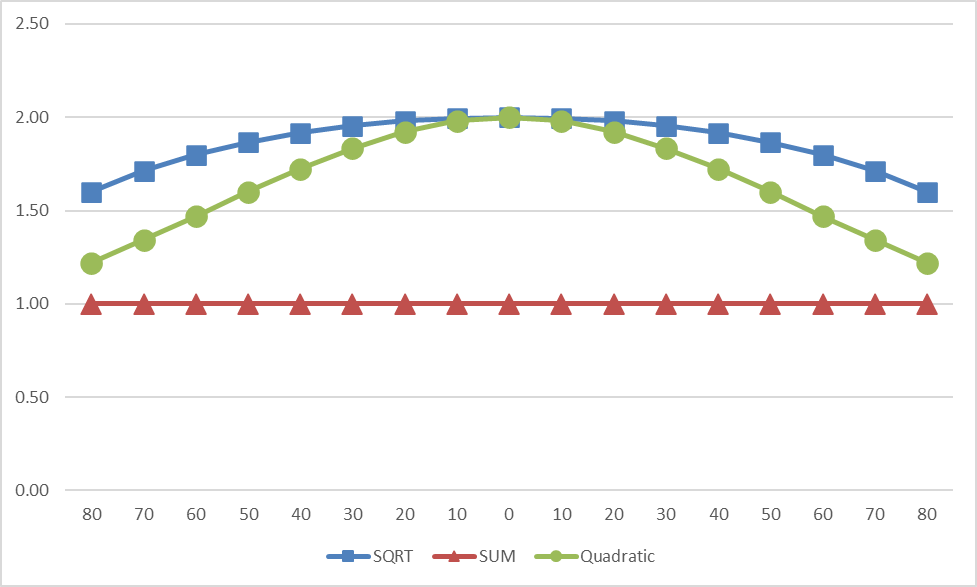
\includegraphics[width=0.8\columnwidth]{1.png}
    \caption{
    تفاوت رابطه درجه دوم، رادیکالی و ساده به ازای توزیع‌های مختلف }
    \label{g4}
    \end{figure}
    
علاوه بر بحث توزیع مالکیت تعداد مالکان مشترک نیز در ارتباط دو نماد می‌تواند تاثیر گذار باشد. به جهت بررسی نحوه تغییر سه رابطه از جهت تعداد مالکان و تمرکز مالکیت در جدول 
\ref{t11}
و 
\ref{t12}
دو مثال بیان شده‌است. در این محاسبات دو نماد x
و
y 
وجود دارد که  در محاسبات جدول 
\ref{t11}
دارای دو سهامدار مشترک می‌باشند. همانطور که انتظار داشتیم با توجه به شکل 
\ref{g4}
به ازای یکسان بودن مالکیت دو سهامدار هر دو عامل عدد دو را نشان می‌دهند و هر آنچه تفاوت مالکیت دو مالک افزایش پیدا کند این دو رابطه کاهش می‌یابند. البته رابطه درجه دوم با افزایش اختلاف، مقدار بیشتری کاهش پیدا می‌کند که با دریافت ما از نمودار شکل 
\ref{g4}
سازگار است. نتایج فوق در جدول 
\ref{t12}
برای دو سهام دارای سه سهامدار مشترک محاسبه شده‌است و نتایج مانند حالت قبل بدست آمده‌است.

در این دو مثال در سه ستون اول تمام مالکیت دو نماد در اختیار سهامداران مشترک می‌باشد ولی در دنیای واقع امکان دارد صرفا بخشی از مالکیت میان دو نماد به صورت مشترک باشد. از این رو در چهار ستون انتهای دو جدول، ملاک‌های مطرح شده به ازای مالکیت‌ مشترک کمتر از صد درصد بررسی شده‌است. در این قسمت مقادیر محاسبه شده توسط رابطه درجه دوم از رشد چشم گیری برخوردار می‌باشد که به نظر می‌آید خلاف ارتباط دو نماد باشد. در واقع مالکیت مشترک دو نماد کاهش چشم گیری پیدا کرده است ولی ملاک ارتباط دو نماد بر اساس رابطه درجه دوم افزایش قابل توجهی داشته‌است. از طرفی رابطه رادیکالی در این کاهش مالکیت به صورت متناسی کاهش پیدا می‌کند و این امر قابل قبول است.




  \begin{table}[htbp]
    \centering
    
\begin{LTR} \lr{          \begin{tabular}{|c|ccc|cccc|}
 \hline
              & Percent & Percent & Percent & Percent & Percent & Percent & Percent \\
              \hline
 x1    & 50    & 20    & 10    & 5     & 10    & 20    & 1 \\
           y1    & 50    & 80    & 90    & 5     & 10    & 20    & 1 \\
            \hline
 x2    & 50    & 80    & 90    & 5     & 10    & 20    & 1 \\
 y2    & 50    & 20    & 10    & 5     & 10    & 20    & 1 \\
           \hline
 SQRT  & 2     & 1.8   & 1.6   & 0.2   & 0.4   & 0.8   & 0.04 \\
 SUM   & 1     & 1     & 1     & 0.1   & 0.2   & 0.4   & 0.02 \\
 Quadratic & 2     & 1.47 & 1.21 & 200   & 50    & 12.5  & 5000 \\
           \cline{1-8}
     \end{tabular}}
     \end{LTR}
     \caption{مثال شماره 1. دو نماد دارای دو سهامدار مشترک}
         \label{t11}
  \end{table}%}

  

  \begin{table}[htbp]
    \centering
 \begin{LTR}\lr{\begin{tabular}{|c|ccc|cccc|}
 \hline
             & Percent & Percent & Percent & Percent & Percent & Percent & Percent \\
             \hline
       x1    & 33.33 & 10    & 20    & 5     & 10    & 20    & 1 \\
       y1    & 33.33 & 10    & 10    & 5     & 10    & 20    & 1 \\
        \hline
       x2    & 33.33 & 80    & 10    & 5     & 10    & 20    & 1 \\
       y2    & 33.33 & 80    & 20    & 5     & 10    & 20    & 1 \\
       \hline
       x3    & 33.33 & 10    & 70    & 5     & 10    & 20    & 1 \\
       y3    & 33.33 & 10    & 70    & 5     & 10    & 20    & 1 \\
       \hline
       SQRT  & 3     & 2.33 & 2.56 & 0.45  & 0.9   & 1.8   & 0.09 \\
       SUM   & 1     & 1     & 1     & 0.15  & 0.3   & 0.6   & 0.03 \\
       Quadratic & 3     & 1.51 & 1.85 & 133.33 & 33.33 & 8.33 & 3333.33 \\
       \hline
       \end{tabular} 
 }\end{LTR}
     \caption{مثال شماره 2. دو نماد دارای سه سهامدار مشترک}
         \label{t12}
           \end{table}%}
  
      %
        
  با توجه به توضیحات انجام شده و نتایج جداول 
  \ref{t11}
  و 
  \ref{t12}
  به نظر می‌آید هر چند رابطه درجه دوم توانایی توضیح دهندگی بهتری از رابطه رادیکالی داشته باشد ولی به دلیل تورش بالا و کیفتیت پایین در مالکیت‌های مشترک پایین، رابطه رادیکالی جهت محاسبه ارتباط دو نماد با توجه به سهامداری مشترک از کیفیت بالاتری برخوردار باشد. 
   در نتیجه در ادامه از رابطه رادیکالی  
           (رابطه \ref{e5}) تحت عنوان 
           $ FCA $
           به عنوان ملاک ارتباط دو نماد استفاده می‌شود.
البته این رابطه توانایی لحاظ تمرکز سهامداری در یک سهامدار را ندارد. برای مثال چنانچه دو نماد، دارای دو سهامدار مشترک باشند و سهامدار شماره یک  $ 80\% $ از هر دو نماد را دارا باشد نتیجه ملاک با حالتی که سهامدار شماره یک از یک نماد $ 20 \% $ و از نماد دیگر $ 80\% $ داشته باشد تفاوتی ندارد.
  
  
  با توجه به تواتر داده‌های موجود، مالکیت مشترک در سه سطح روزانه، هفتگی و ماهانه قابل تعریف می‌باشد. در ادامه جدول خلاصه آماری  برای دو متغیر 
  $ FCA $ 
  (رابطه 
  \ref{e5})
  و 
  $ FCAP $
  (رابطه 
  \ref{e2})
  در جدول 
  \ref{t2}
  و
  \ref{t3}
  ذکر شده‌است. با توجه به مقاله اصلی، جهت استفاده از این پارامتر‌ها از تبدیل رتبه‌ای نرمال شده استفاده شده‌است و در ادامه از این پارامتر تبدیل شده به ترتیب به عنوان 
  $ NFCA$
  و
  $ NFCAP $
  یاد‌شده است. شایان به ذکر است که با توجه به محاسبات آینده در تواتر‌های متفاوت نیز از این متغیر‌ها استفاده شده‌است که برای مثال برای  متغیر 
  $ NFCA$
  تواتر هفتگی آن با پارامتر
  $ NWFCA$
   و ماهانه آن به صورت
   $ NMFCA $
   نشان داده‌شده است. برای متغیر $ NFCAP $ نیز به همین ترتیب با تواتر‌های مختلف استفاده شده‌است.
   
  {\begin{table}[htbp]
    \centering
   \lr{ \begin{LTR}
      \begin{tabular}{l|c|cc|ccccc}
          FCA (\ref{e5})  & {count} & {mean} &{std} &{min} & 25\%  & 50\%  & 75\%  & {max} \\
            \hline                    
    Daily & 8303331 & 0.234 & 0.400 & 0.003 & 0.037 & 0.087 & 0.242 & 11.531 \\
    Weekly & 2418984 & 0.233 & 0.396 & 0.003 & 0.037 & 0.087 & 0.242 & 9.204 \\
    Monthly & 533157 & 0.227 & 0.389 & 0.003 & 0.037 & 0.085 & 0.235 & 7.934 \\
    \end{tabular}%}
      \end{LTR}}
        \caption{خلاصه آماری پارامتر 
        FCA
        در تواتر‌های مختلف  }
        \label{t2}
  \end{table}}
  
  
   {\begin{table}[htbp]
     \centering
    \lr{ \begin{LTR}
       \begin{tabular}{l|c|cc|ccccc}
         FCAP (\ref{e2})  & {count} & {mean} &{std} &{min} & 25\%  & 50\%  & 75\%  & {max} \\
             \hline                    
    Daily & 8303331 & 0.203 & 0.292 & 0.002 & 0.035 & 0.084 & 0.230 & 2.800 \\
    Weekly & 2418984 & 0.202 & 0.290 & 0.002 & 0.035 & 0.084 & 0.230 & 2.535 \\
    Monthly & 533157 & 0.198 & 0.284 & 0.003 & 0.035 & 0.083 & 0.224 & 2.213 \\
     \end{tabular}%}
       \end{LTR}}
         \caption{خلاصه آماری پارامتر 
                 FCAP
                 در تواتر‌های مختلف  }
         \label{t3}
   \end{table}} 
  
  \subsection{محاسبه هم‌بستگی دو نماد}
 با استفاده از قیمت پایانی نماد در هر روز بازده روزانه هر سهم محاسبه می‌شود.
 از آنجا كه  هم بستگی دو نماد براساس بازده روزانه محاسبه می‌شود نیاز است تا عوامل برونزا که می‌توانند سبب هم‌بستگی میان دو نماد گردند کنترل شوند. از این رو همانند مقاله بخش 
\ref{s1.1}
از مدل چهارعاملی کارهارت 
\LTRfootnote{\lr{Carhart four-factor model}}
برای حذف عوامل برونزا استفاده شده‌است. ابتدا برای هر نماد ضرایب عوامل در کل بازه محاسبه می‌شود و پس از آن باقی مانده مدل چهارعاملی برای هر روز محاسبه می‌شود. رابطه 
\ref{e7}
باقی‌مانده 
$ u _{t,i} $
را با حذف عوامل برونزا محاسبه می‌کند.
 
  \begin{align}
  { R_{t,i}=\alpha _{i}+\beta _{mkt,i}{\mathit {R}}_{MKT,t}+\beta _{HML,i}{\mathit {HML}}_{t}+\beta _{SMB,i}{\mathit {SMB}}_{t}+\beta _{UMD,i}{\mathit {UMD}}_{t}+u _{t,i}}
  \label{e6}\\
  u _{t,i} = R_{t,i} - \hat{\alpha} _{i}-\hat{\beta} _{mkt,i}{\mathit {R}}_{MKT,t}-\hat{\beta} _{HML,i}{\mathit {HML}}_{t}-\hat{\beta} _{SMB,i}{\mathit {SMB}}_{t}-\hat{\beta} _{UMD,i}{\mathit {UMD}}_{t}
   \label{e7}
  \end{align}
  
  جهت محاسبه هم‌بستگی میان دو نماد از هم‌بستگی باقی‌مانده‌ روزانه  دو جفت استفاده‌شده است. هم‌بستگی دو نماد نیز در تواتر هفتگی و ماهانه محاسبه شده‌است. در جدول 
  \ref{t4}
  خلاصه آماری هم‌بستگی جفت‌های مختلف بیان شده‌است. در شکل 
  \ref{f1}
  و
  \ref{f2}
  نمودار رابطه هم‌بستگی خطی و ملاک ارتباط دو نماد نیز در تواتر‌های هفتگی و ماهانه   با جدا سازی نماد‌های هم‌گروه و غیر‌هم‌گروه نشان‌داده شده‌است. همانطور که انتظار داشتیم هر آنچه ارتباط دو نماد افزایش پیدا می‌کند بازده دو نماد نیز مرتبط‌تر می‌شود.
  
   {\begin{table}[htbp]
     \centering
    \lr{ \begin{LTR}
       \begin{tabular}{l|c|cc|ccccc}
           $ \rho_{ij,t} $  & {count} & {mean} &{std} &{min} & 25\%  & 50\%  & 75\%  & {max} \\
             \hline 
    Weekly & 2296671 & 0.05  & 0.63  & -1    & -0.49 & 0.08  & 0.62  & 1 \\
    Monthly & 525626 & 0.05  & 0.36  & -1    & -0.17 & 0.05  & 0.28  & 1 \\
     \end{tabular}%}
       \end{LTR}}
         \caption{خلاصه آماری پارامتر هم‌بستگی خطی   }
         \label{t4}
   \end{table}} 
  
  
  \begin{figure}[htbp]
  \centering
  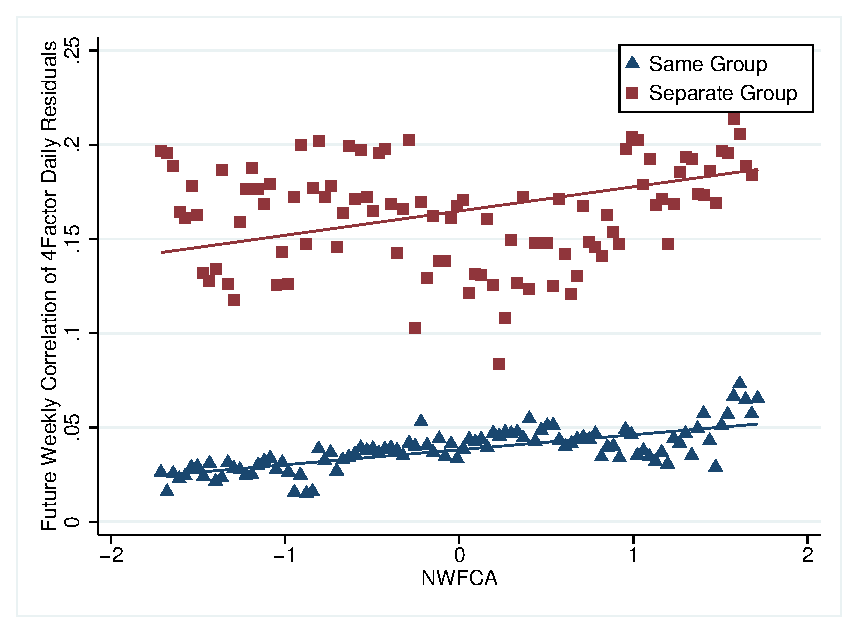
\includegraphics[width=.70\linewidth]{wcorr.eps}
    \caption{نمودار 
        $ \rho_{ij,{t+1}} $
        هفتگی  بر روی 
    $ NWFCA $ 
    به تفکیک یکسان بودن گروه کسب و کار}
    \label{f1}
  \end{figure}
  
  \begin{figure}[htbp]
  \centering
  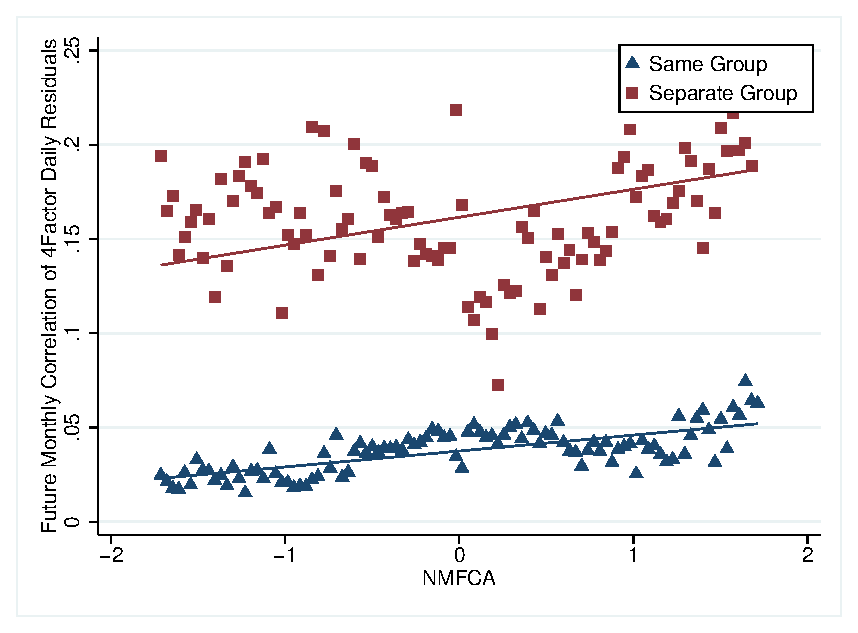
\includegraphics[width=.70\linewidth]{mcorr.eps}
    \caption{نمودار 
    $ \rho_{ij,{t+1}} $
    ماهانه 
    بر روی 
    $ NMFCA $ 
     به تفکیک یکسان بودن گروه کسب و کار}
    \label{f2}
  \end{figure}
  
  \FloatBarrier
  
  
  \subsection{مدل‌سازی هم‌حرکتی دو نماد}
  جهت بررسی اثر مالکیت مشترک بر هم حرکتی دو نماد از رابطه 
  \ref{e8}
  استفاده شده است. در این رابطه منظور از
   $ \text{Factor }_{ij,t} $
    معیار ارتباط دو نماد می‌باشد که پس از محاسبه به وسیله  رابطه‌های 
   \ref{e2}
   و
   \ref{e5}
   تبدیل رتبه‌ای نرمال شده بر روی آن اعمال شده‌است. از این مدل در تواتر‌های ماهانه و هفتگی جهت برآورد ضریب $ b_f $ استفاده شده‌است.
   
  
    \begin{equation}
    \rho_{ij,t+1} = a + b_f \times \text{Factor }_{ij,t} + \sum_{k = 1}^{n } CONTROL_{ij,t,k} + \varepsilon_{ij,t+1}
    \label{e8}
    \end{equation}
  
در این مدل  علاوه بر از بین بردن روند‌های موجود در بازده سهام به وسیله مدل چهارعاملی، از کنترل‌های دیگر نیز استفاده شده‌است.  
جهت کنترل اثر هم‌گروهی بودن دو نماد پارامتر  
  $ \text{sgroup} $
  تعریف شده‌است  تا چنانچه دو سهم به یک گروه صنعتی تعلق داشته باشند آنگاه مقدار آن برابر یک شود. از طرفی یکی دیگر از عوامل تاثیر گذار در رفتار مشابه دو نماد اندازه بازار دو نماد می‌باشد که جهت کنترل یکسان بودن اندازه دو سهم پارامتر
  $ \text{samesize} $
 تعریف شده‌است که برابر منفی اختلاف رتبه صدکی اندازه دو سهم می‌باشد. متغیر 
  $ \text{size} $ 
  نیز رتبه صدکی اندازه سهم می‌باشد که در کلیه جداول منظور از 
  شرکت 1 شرکت بزرگتر است. یکی دیگر از کنترل‌های مورد استفاده هم بستگی در دوره‌ی $ t $ می‌باشد. برای محاسبه متغیر‌های کنترل و وابسته در تواتر‌های هفتگی و ماهانه از میانگین این متغیر‌ها در بازه مورد نظر استفاده شده‌است.
  خلاصه آماری پارامتر‌های تعریف شده در جدول 
  \ref{t5}
  و 
  \ref{t6}
  نشان داده شده‌است.
  
  
  
  
  
  
  
     {\begin{table}[htbp]
       \centering
      \lr{ \begin{LTR}
    \begin{tabular}{l|cc|cccccc}
          & count & mean  & std   & min   & 25\%  & 50\%  & 75\%  & max \\
          \hline
    WSizeRatio & 2418984 & 6.836 & 34.394 & 0.000 & 0.230 & 0.898 & 3.119 & 11184.040 \\
    Wsize1 & 2418984 & 0.733 & 0.220 & 0.006 & 0.585 & 0.788 & 0.921 & 1 \\
    Wsize2 & 2418984 & 0.450 & 0.256 & 0.002 & 0.244 & 0.429 & 0.646 & 1\\
    WSameSize & 2418984 & -0.284 & 0.218 & -0.994 & -0.424 & -0.238 & -0.102 & 0.447 \\
    sgroup & 2418984 & 0.126 & 0.332 & 0     & 0     & 0     & 0     & 1 \\
    \end{tabular}%
         \end{LTR}}
           \caption{خلاصه آماری پارامتر‌های هفتگی   }
           \label{t5}
     \end{table}} 

     \FloatBarrier
 
 
\section{یافته‌های پژوهش}
در این قسمت از تواتر هفتگی متغیر‌ها جهت بررسی اثر ارتباط دو نماد از طریق سهامدار مشترک استفاده می‌شود. نتایج مدل با داده‌های ماهانه در ضمیمه 
\ref{sa.1}
آورده شده‌است.
بعد از محاسبه متغیر‌ها با توجه به توضیحات گذشته، در ابتدا به روش مقاله  بخش 
\ref{s1.1}
از روش فاما مکبث 1973 
\LTRfootnote{Fama and MacBeth 1973}
ضرایب را تخمین می‌زنیم. در جدول 
\ref{t7} 
نتایج این برآورد  
برای حالت‌های مختلف آورده شده‌است. همانند مقاله بخش 
\ref{s1.1}
در همه‌ی حالت‌ها ضریب برآورد شده معنا‌دار می‌باشد. در ستون اول این جدول از نسخه ساده شده مدل 
\ref{e8}
استفاده شده‌است. در این حالت ارتباط معنا‌داری میان هم بستگی آینده بازده قیمتی و ارتباط دو نماد وجود دارد. جهت کنترل عوامل نادیده گرفته شده از هم‌بستگی دوره t استفاده شده‌است. در ستون (3) نیز متغیر‌های کنترل کننده یکسان بودن گروه صنعتی و اندازه دو نماد اضافه شده‌است که پس از کنترل هم بستگی دوره قبل و هم‌گروهی دو نماد، این عامل بیشترین تاثیر را در هم‌بستگی خطی میان رفتار بازده دو نماد می‌گذارد. با افزایش نزدیکی اندازه دو نماد، نیز هم بستگی خطی میان دو نماد افزایش پیدا می‌کند. در مدل‌های (4) و (6) کنترل اندازه دو نماد نیز به مدل اضافه شده‌است که به نظر می‌آید هرآنچه شرکت بزرگتر، کوچک شود و شرکت کوچک بزرگ شود هم بستگی خطی میان دو نماد افزایش پیدا می‌کند. 

در جدول 
\ref{t8}
نتایج برآورد ضرایب مدل به روش حداقل مربعات معمولي و با
دسته بندی در سطح جفت‌های مشترک، جهت محاسبه خطاي استاندارد ضرايب آورده شده‌است. در این برآورد نیز کلیه ضرایب مورد بررسی، معنادار می‌باشند و با نتایج روش فاما مکبث سازگار می‌باشند.  در مقاله مورد بحث داده‌های مالکیت به صورت فصلی موجود بوده‌است و تواتر داده‌های هم‌بستگی به صورت ماهانه می‌باشد. با توجه به موجود بودن داده‌ مالکیت در تواتر هفتگی و ماهانه از این رو به نظر می‌رسد استفاده از روش حداقل مربعات قابل قبول باشد.

نتایج برآورد به دو روش حداقل مربعات و فاما مکبث در تواتر ماهانه در ضمایم
\ref{sa.1}
آورده شده‌است که نشان می‌دهد که نتایج به انتخاب تواتر بستگی ندارد.
 در ضمیمه 
\ref{sa.2}
نیز برآورد‌های متفاوت با استفاده از روش‌ها و پارامتر‌های متفاوت سنجی آورده شده‌است که نتایج فوق تایید شده‌اند.

\nopagebreak

% & \multicolumn{6}{c}{Dependent Variable: Weekly Correlation of 4F Residuals}                 \\
% \cline{2-7}


\begin{table}[htbp]
\centering
\begin{LTR}
\lr{{
\def\sym#1{\ifmmode^{#1}\else\(^{#1}\)\fi}
\begin{tabular}{l*{7}{c}}
\hline\hline
 & \multicolumn{7}{c}{Dependent Variable: Fortnightly Correlation of 4F+Industry Residuals}                 \\
 \cline{2-8}
                    &\multicolumn{1}{c}{(1)}         &\multicolumn{1}{c}{(2)}         &\multicolumn{1}{c}{(3)}         &\multicolumn{1}{c}{(4)}         &\multicolumn{1}{c}{(5)}         &\multicolumn{1}{c}{(6)}         &\multicolumn{1}{c}{(7)}         \\
\hline
FCA*          &     0.00830\sym{***}&     0.00827\sym{***}&     0.00563\sym{***}&     0.00358\sym{***}&     0.00314\sym{***}&     0.00323\sym{***}&     0.00314\sym{***}\\
                    &      (7.88)         &      (7.83)         &      (8.37)         &      (6.64)         &      (6.69)         &      (6.82)         &      (6.69)         \\
[1em]
${\text{FCA}^*}^2 $    &                     &     0.00871\sym{***}&     0.00629\sym{***}&     0.00490\sym{***}&     0.00525\sym{***}&     0.00524\sym{***}&     0.00525\sym{***}\\
                    &                     &     (12.49)         &     (13.89)         &     (11.15)         &     (11.53)         &     (11.56)         &     (11.61)         \\
[1em]
$ \rho\_t $          &                     &                     &       0.279\sym{***}&       0.278\sym{***}&       0.277\sym{***}&       0.277\sym{***}&       0.277\sym{***}\\
                    &                     &                     &     (15.87)         &     (15.86)         &     (15.91)         &     (15.91)         &     (15.91)         \\
[1em]
sgroup              &                     &                     &                     &      0.0190\sym{***}&      0.0174\sym{***}&      0.0173\sym{***}&      0.0175\sym{***}\\
                    &                     &                     &                     &      (8.08)         &      (7.78)         &      (7.71)         &      (7.77)         \\
[1em]
Samesize            &                     &                     &                     &     -0.0179\sym{***}&                     &     -0.0321\sym{***}&                     \\
                    &                     &                     &                     &     (-6.21)         &                     &     (-5.35)         &                     \\
[1em]
Size1               &                     &                     &                     &                     &     -0.0400\sym{***}&                     &     -0.0412\sym{***}\\
                    &                     &                     &                     &                     &     (-5.05)         &                     &     (-4.29)         \\
[1em]
Size2               &                     &                     &                     &                     &     0.00979\sym{***}&                     &     0.00647         \\
                    &                     &                     &                     &                     &      (4.39)         &                     &      (0.60)         \\
[1em]
$ Size1 \times Size2 $&                     &                     &                     &                     &                     &     -0.0255\sym{***}&     0.00393         \\
                    &                     &                     &                     &                     &                     &     (-4.25)         &      (0.33)         \\
[1em]
Constant            &      0.0130\sym{***}&     0.00438\sym{**} &     0.00308\sym{**} &     0.00707\sym{***}&      0.0273\sym{***}&      0.0208\sym{***}&      0.0283\sym{***}\\
                    &      (7.68)         &      (2.95)         &      (2.89)         &      (4.50)         &      (4.21)         &      (4.31)         &      (3.55)         \\
\hline
Observations        &     1405333         &     1405333         &     1379678         &     1379678         &     1379678         &     1379678         &     1379678         \\
\(R^{2}\)           &       0.001         &       0.001         &       0.240         &       0.241         &       0.242         &       0.242         &       0.242         \\
\hline\hline
\multicolumn{8}{l}{\footnotesize \textit{t} statistics in parentheses}\\
\multicolumn{8}{l}{\footnotesize This table reports Fama and MacBeth (1973) estimates of fortnightly cross-sectional}\\
\multicolumn{8}{l}{\footnotesize  regressions forecasting the correlation of daily 4Factor+Industry residuals in fortnight t + 1 for each pairs.}\\
\multicolumn{8}{l}{\footnotesize The independent variables are updated fortnightly and include our measure of institutional connectedness,}\\
\multicolumn{8}{l}{\footnotesize  FCA and a series of controls at time t.}\\
\multicolumn{8}{l}{\footnotesize We measure the negative of the absolute value of the difference in size ranking across the two stocks in the pair $ \text{Samesize}\_{ij,t} $.}\\
\multicolumn{8}{l}{\footnotesize We also capture the similarity in business group by dummy of sgroup.}\\
\multicolumn{8}{l}{\footnotesize Independent variables which  we denote with * are rank-transformed and normalized to have unit standard deviation.}\\
\multicolumn{8}{l}{\footnotesize  We calculate Newey and West (1987) standard errors (four lags) of the Fama and MacBeth (1973) estimates }\\
\multicolumn{8}{l}{\footnotesize  that take into account autocorrelation in the cross-sectional slopes}\\
\multicolumn{8}{l}{\footnotesize \sym{*} \(p<0.05\), \sym{**} \(p<0.01\), \sym{***} \(p<0.001\)}\\
\end{tabular}
}
}
\end{LTR}
\caption{برآورد به روش فاما مکبث 1973}
\label{t7}
\end{table}


% & \multicolumn{6}{c}{Dependent Variable: Weekly Correlation of 4F Residuals}                 \\
% \cline{2-7}


\begin{table}[htbp]
\centering
\begin{LTR}
\lr{{
\def\sym#1{\ifmmode^{#1}\else\(^{#1}\)\fi}
\begin{tabular}{l*{6}{c}}
\hline\hline
 & \multicolumn{6}{c}{Dependent Variable: Weekly Correlation of 4F Residuals}                 \\
 \cline{2-7}
                    &\multicolumn{1}{c}{(1)}         &\multicolumn{1}{c}{(2)}         &\multicolumn{1}{c}{(3)}         &\multicolumn{1}{c}{(4)}         &\multicolumn{1}{c}{(5)}         &\multicolumn{1}{c}{(6)}         \\
\hline
WeeklyFCA*          &      0.0192\sym{***}&      0.0160\sym{***}&     0.00626\sym{***}&     0.00558\sym{***}&     0.00580\sym{***}&     0.00642\sym{***}\\
                    &     (17.97)         &     (18.12)         &      (8.21)         &      (7.51)         &      (7.86)         &      (8.72)         \\
[1em]
WCorr               &                     &       0.184\sym{***}&       0.180\sym{***}&       0.179\sym{***}&       0.179\sym{***}&       0.179\sym{***}\\
                    &                     &    (195.32)         &    (206.88)         &    (204.85)         &    (204.47)         &    (204.27)         \\
[1em]
sgroup              &                     &                     &       0.105\sym{***}&       0.101\sym{***}&       0.100\sym{***}&      0.0992\sym{***}\\
                    &                     &                     &     (33.23)         &     (32.05)         &     (31.66)         &     (31.22)         \\
[1em]
WSamesize           &                     &                     &      0.0539\sym{***}&                     &      0.0972\sym{***}&                     \\
                    &                     &                     &     (16.60)         &                     &     (29.57)         &                     \\
[1em]
WSize1              &                     &                     &                     &      -0.115\sym{***}&                     &     -0.0463\sym{***}\\
                    &                     &                     &                     &    (-31.09)         &                     &     (-8.63)         \\
[1em]
WSize2              &                     &                     &                     &      0.0281\sym{***}&                     &       0.244\sym{***}\\
                    &                     &                     &                     &      (7.99)         &                     &     (19.00)         \\
[1em]
wsize1size2         &                     &                     &                     &                     &     -0.0836\sym{***}&      -0.253\sym{***}\\
                    &                     &                     &                     &                     &    (-25.92)         &    (-16.70)         \\
\hline
Observations        &     2280984         &     2189145         &     2189145         &     2189145         &     2189145         &     2189145         \\
\hline\hline
\multicolumn{7}{l}{\footnotesize \textit{t} statistics in parentheses}\\
\multicolumn{7}{l}{\footnotesize \sym{*} \(p<0.05\), \sym{**} \(p<0.01\), \sym{***} \(p<0.001\)}\\
\end{tabular}
}
}
\end{LTR}
\caption{برآورد به روش حداقل مربعات با محاسبه واریانس با دسته بندی در سطح جفت}
\label{t8}
\end{table}



% & \multicolumn{6}{c}{Dependent Variable: Monthly Correlation of 4F Residuals}                 \\
% \cline{2-7}
  \begin{table}[htbp]
  \centering
  \begin{LTR}
  \lr{{
\def\sym#1{\ifmmode^{#1}\else\(^{#1}\)\fi}
\begin{tabular}{l*{6}{c}}
\hline\hline
 & \multicolumn{6}{c}{Dependent Variable: Monthly Correlation of 4F Residuals}                 \\
 \cline{2-7}
                    &\multicolumn{1}{c}{(1)}         &\multicolumn{1}{c}{(2)}         &\multicolumn{1}{c}{(3)}         &\multicolumn{1}{c}{(4)}         &\multicolumn{1}{c}{(5)}         &\multicolumn{1}{c}{(6)}         \\
\hline
WeeklyFCA*          &      0.0188\sym{***}&      0.0159\sym{***}&     0.00527\sym{***}&     0.00374\sym{***}&     0.00397\sym{***}&     0.00467\sym{***}\\
                    &     (36.04)         &     (35.64)         &     (15.35)         &     (11.59)         &     (12.20)         &     (13.71)         \\
[1em]
WCorr               &                     &       0.148\sym{***}&       0.143\sym{***}&       0.141\sym{***}&       0.140\sym{***}&       0.140\sym{***}\\
                    &                     &     (37.95)         &     (37.22)         &     (38.39)         &     (38.40)         &     (38.38)         \\
[1em]
sgroup              &                     &                     &       0.112\sym{***}&       0.108\sym{***}&       0.107\sym{***}&       0.105\sym{***}\\
                    &                     &                     &     (53.99)         &     (52.38)         &     (52.03)         &     (52.05)         \\
[1em]
WSamesize           &                     &                     &      0.0427\sym{***}&                     &       0.101\sym{***}&                     \\
                    &                     &                     &     (16.70)         &                     &     (18.91)         &                     \\
[1em]
WSize1              &                     &                     &                     &      -0.125\sym{***}&                     &     -0.0468\sym{***}\\
                    &                     &                     &                     &    (-19.10)         &                     &     (-8.99)         \\
[1em]
WSize2              &                     &                     &                     &      0.0111\sym{***}&                     &       0.255\sym{***}\\
                    &                     &                     &                     &      (5.83)         &                     &     (15.65)         \\
[1em]
wsize1size2         &                     &                     &                     &                     &      -0.107\sym{***}&      -0.284\sym{***}\\
                    &                     &                     &                     &                     &    (-20.80)         &    (-15.92)         \\
\hline
Observations        &     2392368         &     2277130         &     2277130         &     2277130         &     2277130         &     2277130         \\
\hline\hline
\multicolumn{7}{l}{\footnotesize \textit{t} statistics in parentheses}\\
\multicolumn{7}{l}{\footnotesize \sym{*} \(p<0.05\), \sym{**} \(p<0.01\), \sym{***} \(p<0.001\)}\\
\end{tabular}
}
}
  \end{LTR}
  \caption{برآورد به روش فاما مکبث 1973 }
  \label{t14}
  \end{table}



\FloatBarrier






\begin{appendices}





\section{نتایج برآورد براساس روش‌های مختلف سنجی}
\label{sa.2}
 
 
 \begin{table}[htbp]
 \centering
 \begin{LTR}
 \lr{{
\def\sym#1{\ifmmode^{#1}\else\(^{#1}\)\fi}
\begin{tabular}{l*{6}{c}}
\hline\hline
 & \multicolumn{6}{c}{Dependent Variable: Weekly Correlation of 4F Residuals}                 \\
 \cline{2-7}
                    &\multicolumn{1}{c}{(1)}         &\multicolumn{1}{c}{(2)}         &\multicolumn{1}{c}{(3)}         &\multicolumn{1}{c}{(4)}         &\multicolumn{1}{c}{(5)}         &\multicolumn{1}{c}{(6)}         \\
\hline
FCA*                &      0.0193\sym{***}&     0.00468\sym{***}&     0.00167\sym{***}&     0.00129\sym{***}&     0.00134\sym{***}&     0.00148\sym{***}\\
                    &     (49.90)         &     (16.78)         &      (8.70)         &      (7.21)         &      (7.46)         &      (8.15)         \\
[1em]
WCorr               &                     &       0.755\sym{***}&       0.753\sym{***}&       0.753\sym{***}&       0.753\sym{***}&       0.752\sym{***}\\
                    &                     &     (74.81)         &     (74.23)         &     (73.96)         &     (73.93)         &     (73.91)         \\
[1em]
sgroup              &                     &                     &      0.0316\sym{***}&      0.0304\sym{***}&      0.0302\sym{***}&      0.0300\sym{***}\\
                    &                     &                     &     (20.65)         &     (20.46)         &     (20.41)         &     (20.39)         \\
[1em]
SameSize            &                     &                     &      0.0151\sym{***}&                     &      0.0285\sym{***}&                     \\
                    &                     &                     &     (12.28)         &                     &     (12.64)         &                     \\
[1em]
size1               &                     &                     &                     &     -0.0342\sym{***}&                     &     -0.0175\sym{***}\\
                    &                     &                     &                     &    (-12.18)         &                     &     (-7.12)         \\
[1em]
size2               &                     &                     &                     &     0.00804\sym{***}&                     &      0.0597\sym{***}\\
                    &                     &                     &                     &      (7.62)         &                     &      (9.65)         \\
[1em]
size1size2          &                     &                     &                     &                     &     -0.0243\sym{***}&     -0.0601\sym{***}\\
                    &                     &                     &                     &                     &    (-10.37)         &     (-8.61)         \\
\hline
Observations        &     8165331         &     8073492         &     8073492         &     8073492         &     8073492         &     8073492         \\
\hline\hline
\multicolumn{7}{l}{\footnotesize \textit{t} statistics in parentheses}\\
\multicolumn{7}{l}{\footnotesize \sym{*} \(p<0.05\), \sym{**} \(p<0.01\), \sym{***} \(p<0.001\)}\\
\end{tabular}
}
}
 \end{LTR}
 \caption{نتایج برآورد به روش فاما مکبت با استفاده از هم‌بستگی هفتگی و پارامتر‌های کنترلی روزانه}
 \label{t13}
 \end{table}
 

 \begin{table}[htbp]
  \centering
  \begin{LTR}
  \lr{{
\def\sym#1{\ifmmode^{#1}\else\(^{#1}\)\fi}
\begin{tabular}{l*{6}{c}}
\hline\hline
 & \multicolumn{6}{c}{Dependent Variable: Weekly Correlation of 4F Residuals}                 \\
 \cline{2-7}
                    &\multicolumn{1}{c}{(1)}         &\multicolumn{1}{c}{(2)}         &\multicolumn{1}{c}{(3)}         &\multicolumn{1}{c}{(4)}         &\multicolumn{1}{c}{(5)}         &\multicolumn{1}{c}{(6)}         \\
\hline
FCA*                &      0.0193\sym{***}&     0.00468\sym{***}&     0.00167\sym{***}&     0.00129\sym{***}&     0.00134\sym{***}&     0.00148\sym{***}\\
                    &     (49.90)         &     (16.78)         &      (8.70)         &      (7.21)         &      (7.46)         &      (8.15)         \\
[1em]
WCorr               &                     &       0.755\sym{***}&       0.753\sym{***}&       0.753\sym{***}&       0.753\sym{***}&       0.752\sym{***}\\
                    &                     &     (74.81)         &     (74.23)         &     (73.96)         &     (73.93)         &     (73.91)         \\
[1em]
sgroup              &                     &                     &      0.0316\sym{***}&      0.0304\sym{***}&      0.0302\sym{***}&      0.0300\sym{***}\\
                    &                     &                     &     (20.65)         &     (20.46)         &     (20.41)         &     (20.39)         \\
[1em]
SameSize            &                     &                     &      0.0151\sym{***}&                     &      0.0285\sym{***}&                     \\
                    &                     &                     &     (12.28)         &                     &     (12.64)         &                     \\
[1em]
size1               &                     &                     &                     &     -0.0342\sym{***}&                     &     -0.0175\sym{***}\\
                    &                     &                     &                     &    (-12.18)         &                     &     (-7.12)         \\
[1em]
size2               &                     &                     &                     &     0.00804\sym{***}&                     &      0.0597\sym{***}\\
                    &                     &                     &                     &      (7.62)         &                     &      (9.65)         \\
[1em]
size1size2          &                     &                     &                     &                     &     -0.0243\sym{***}&     -0.0601\sym{***}\\
                    &                     &                     &                     &                     &    (-10.37)         &     (-8.61)         \\
\hline
Observations        &     8165331         &     8073492         &     8073492         &     8073492         &     8073492         &     8073492         \\
\hline\hline
\multicolumn{7}{l}{\footnotesize \textit{t} statistics in parentheses}\\
\multicolumn{7}{l}{\footnotesize \sym{*} \(p<0.05\), \sym{**} \(p<0.01\), \sym{***} \(p<0.001\)}\\
\end{tabular}
}
} ‌ ‌ %WOresult
  \end{LTR}
  \caption{نتایج برآورد ضرایب به روش 
  OLS 
  ،
  Tobit
  و
  ML
  و با
  هزار بار تكرار بوت استرپ، خطاي استاندارد ضرايب محاسبه شده‌است. }
  \label{t16}
  \end{table}
 
 \FloatBarrier
 
 \section{نتایج و جداول ماهانه}
 \label{sa.1}
       \begin{table}[htbp]
         \centering
        \lr{ \begin{LTR}
     \begin{tabular}{l|cc|cccccc}
               & count & mean  & std   & min   & 25\%  & 50\%  & 75\%  & max \\
               \hline
     MSizeRatio & 533157 & 6.915 & 37.306 & 0.000 & 0.233 & 0.907 & 3.136 & 10658.021 \\
     Msize1 & 533157 & 0.729 & 0.222 & 0.006 & 0.579 & 0.782 & 0.918 & 1 \\
     Msize2 & 533157 & 0.444 & 0.256 & 0.002 & 0.240 & 0.422 & 0.640 & 1 \\
     MSameSize & 533157 & -0.285 & 0.218 & -0.992 & -0.425 & -0.239 & -0.103 & 0.410 \\
     sgroup & 533157 & 0.126 & 0.332 & 0     & 0     & 0     & 0     & 1 \\
     \end{tabular}%         
           \end{LTR}}
             \caption{خلاصه آماری پارامتر‌های ماهانه   }
             \label{t6}
       \end{table}
  
 
 \begin{table}[htbp]
 \centering
 \begin{LTR}
 \lr{{
\def\sym#1{\ifmmode^{#1}\else\(^{#1}\)\fi}
\begin{tabular}{l*{7}{c}}
\hline\hline
                    &\multicolumn{1}{c}{(1)}         &\multicolumn{1}{c}{(2)}         &\multicolumn{1}{c}{(3)}         &\multicolumn{1}{c}{(4)}         &\multicolumn{1}{c}{(5)}         &\multicolumn{1}{c}{(6)}         &\multicolumn{1}{c}{(7)}         \\
\hline
$ \text{FCA*} $     &     0.00761\sym{***}&     0.00788\sym{***}&     0.00742\sym{***}&     0.00538\sym{***}&     0.00470\sym{***}&     0.00482\sym{***}&     0.00468\sym{***}\\
                    &      (6.02)         &      (6.06)         &      (6.50)         &      (7.00)         &      (7.75)         &      (7.85)         &      (7.69)         \\
[1em]
$ { \text{FCA}^ * } ^ 2$&                     &     0.00594\sym{***}&     0.00564\sym{***}&     0.00444\sym{***}&     0.00493\sym{***}&     0.00493\sym{***}&     0.00493\sym{***}\\
                    &                     &      (9.16)         &      (9.88)         &      (7.93)         &      (8.73)         &      (8.69)         &      (8.71)         \\
[1em]
 $ \rho\_t $         &                     &                     &      0.0504\sym{***}&      0.0496\sym{***}&      0.0476\sym{***}&      0.0477\sym{***}&      0.0477\sym{***}\\
                    &                     &                     &      (6.71)         &      (7.01)         &      (8.20)         &      (8.11)         &      (8.16)         \\
[1em]
sgroup              &                     &                     &                     &      0.0177\sym{***}&      0.0154\sym{***}&      0.0151\sym{***}&      0.0154\sym{***}\\
                    &                     &                     &                     &      (4.83)         &      (5.04)         &      (4.98)         &      (5.03)         \\
[1em]
Samesize            &                     &                     &                     &      0.0207\sym{***}&                     &      0.0423\sym{**} &                     \\
                    &                     &                     &                     &      (4.12)         &                     &      (3.34)         &                     \\
[1em]
Size1               &                     &                     &                     &                     &     -0.0536\sym{**} &                     &     -0.0527\sym{**} \\
                    &                     &                     &                     &                     &     (-3.26)         &                     &     (-3.17)         \\
[1em]
Size2               &                     &                     &                     &                     &     0.00897\sym{**} &                     &      0.0123         \\
                    &                     &                     &                     &                     &      (3.13)         &                     &      (1.04)         \\
[1em]
$ Size1 \times Size2 $&                     &                     &                     &                     &                     &     -0.0381\sym{**} &    -0.00371         \\
                    &                     &                     &                     &                     &                     &     (-3.12)         &     (-0.28)         \\
[1em]
Constant            &      0.0135\sym{***}&     0.00779\sym{***}&     0.00715\sym{***}&      0.0119\sym{***}&      0.0419\sym{**} &      0.0325\sym{**} &      0.0411\sym{**} \\
                    &      (5.24)         &      (3.53)         &      (3.63)         &      (4.09)         &      (3.09)         &      (3.14)         &      (2.99)         \\
\hline
Observations        &      479631         &      479631         &      475166         &      475166         &      475166         &      475166         &      475166         \\
\(R^{2}\)           &       0.001         &       0.001         &       0.004         &       0.006         &       0.008         &       0.008         &       0.008         \\
\hline\hline
\multicolumn{8}{l}{\footnotesize \textit{t} statistics in parentheses}\\
\multicolumn{8}{l}{\footnotesize This table reports Fama and MacBeth (1973) estimates of monthly cross-sectional}\\
\multicolumn{8}{l}{\footnotesize  regressions forecasting the correlation of daily 4Factor+Industry residuals in month t + 1 for each pairs.}\\
\multicolumn{8}{l}{\footnotesize The independent variables are updated monthly and include our measure of institutional connectedness,}\\
\multicolumn{8}{l}{\footnotesize  FCA and a series of controls at time t.}\\
\multicolumn{8}{l}{\footnotesize We measure the negative of the absolute value of the difference in size ranking across the two stocks in the pair $ \text{Samesize}\_{ij,t} $.}\\
\multicolumn{8}{l}{\footnotesize We also capture the similarity in business group by dummy of sgroup.}\\
\multicolumn{8}{l}{\footnotesize Independent variables which  we denote with * are rank-transformed and normalized to have unit standard deviation.}\\
\multicolumn{8}{l}{\footnotesize  We calculate Newey and West (1987) standard errors (four lags) of the Fama and MacBeth (1973) estimates }\\
\multicolumn{8}{l}{\footnotesize  that take into account autocorrelation in the cross-sectional slopes}\\
\multicolumn{8}{l}{\footnotesize \sym{*} \(p<0.05\), \sym{**} \(p<0.01\), \sym{***} \(p<0.001\)}\\
\end{tabular}
}
}
 \end{LTR}
 \caption{  برآورد به روش فاما مکبث 1973 با استفاده از هم‌بستگی خطی ماهانه و پارامتر‌های ماهانه}
 \label{t9}
 \end{table}
 
 
 % & \multicolumn{6}{c}{Dependent Variable: Correlation of 4F Residuals}                 \\
 % \cline{2-7}
 
 
 
 \begin{table}[htbp]
 \centering
 \begin{LTR}
 \lr{{
\def\sym#1{\ifmmode^{#1}\else\(^{#1}\)\fi}
\begin{tabular}{l*{6}{c}}
\hline\hline
 & \multicolumn{6}{c}{Dependent Variable: Monthly Correlation of 4F Residuals}                 \\
 \cline{2-7}
                    &\multicolumn{1}{c}{(1)}         &\multicolumn{1}{c}{(2)}         &\multicolumn{1}{c}{(3)}         &\multicolumn{1}{c}{(4)}         &\multicolumn{1}{c}{(5)}         &\multicolumn{1}{c}{(6)}         \\
\hline
MonthlyFCA*         &      0.0198\sym{***}&      0.0177\sym{***}&     0.00753\sym{***}&     0.00672\sym{***}&     0.00700\sym{***}&     0.00785\sym{***}\\
                    &     (18.71)         &     (19.00)         &      (9.17)         &      (8.47)         &      (8.88)         &      (9.99)         \\
[1em]
MCorr               &                     &       0.115\sym{***}&       0.102\sym{***}&      0.0979\sym{***}&      0.0969\sym{***}&      0.0959\sym{***}\\
                    &                     &     (47.25)         &     (48.09)         &     (45.75)         &     (45.16)         &     (44.60)         \\
[1em]
sgroup              &                     &                     &       0.113\sym{***}&       0.110\sym{***}&       0.108\sym{***}&       0.106\sym{***}\\
                    &                     &                     &     (32.41)         &     (31.32)         &     (30.84)         &     (30.15)         \\
[1em]
MSamesize           &                     &                     &      0.0475\sym{***}&                     &      0.0989\sym{***}&                     \\
                    &                     &                     &     (13.53)         &                     &     (27.67)         &                     \\
[1em]
MSize1              &                     &                     &                     &      -0.119\sym{***}&                     &     -0.0329\sym{***}\\
                    &                     &                     &                     &    (-29.52)         &                     &     (-5.63)         \\
[1em]
MSize2              &                     &                     &                     &      0.0151\sym{***}&                     &       0.294\sym{***}\\
                    &                     &                     &                     &      (3.99)         &                     &     (20.74)         \\
[1em]
msize1size2         &                     &                     &                     &                     &      -0.102\sym{***}&      -0.328\sym{***}\\
                    &                     &                     &                     &                     &    (-28.91)         &    (-19.49)         \\
\hline
Observations        &      506541         &      501846         &      501846         &      501846         &      501846         &      501846         \\
\hline\hline
\multicolumn{7}{l}{\footnotesize \textit{t} statistics in parentheses}\\
\multicolumn{7}{l}{\footnotesize \sym{*} \(p<0.05\), \sym{**} \(p<0.01\), \sym{***} \(p<0.001\)}\\
\end{tabular}
}
}
 \end{LTR}
 \caption{برآورد به روش حداقل مربعات با محاسبه واریانس با دسته بندی در سطح جفت}
 \label{t10}
 \end{table}
 
  \begin{table}[htbp]
  \centering
  \begin{LTR}
  \lr{{
\def\sym#1{\ifmmode^{#1}\else\(^{#1}\)\fi}
\begin{tabular}{l*{6}{c}}
\hline\hline
 & \multicolumn{6}{c}{Dependent Variable: Monthly Correlation of 4F Residuals}                 \\
 \cline{2-7}
                    &\multicolumn{1}{c}{(1)}         &\multicolumn{1}{c}{(2)}         &\multicolumn{1}{c}{(3)}         &\multicolumn{1}{c}{(4)}         &\multicolumn{1}{c}{(5)}         &\multicolumn{1}{c}{(6)}         \\
\hline
FCA*                &      0.0193\sym{***}&     0.00115\sym{***}&    0.000405\sym{***}&    0.000302\sym{***}&    0.000320\sym{***}&    0.000368\sym{***}\\
                    &     (72.16)         &      (9.66)         &      (6.23)         &      (5.28)         &      (5.53)         &      (6.04)         \\
[1em]
MCorr               &                     &       0.937\sym{***}&       0.936\sym{***}&       0.935\sym{***}&       0.935\sym{***}&       0.935\sym{***}\\
                    &                     &    (183.12)         &    (179.17)         &    (177.40)         &    (177.14)         &    (176.86)         \\
[1em]
sgroup              &                     &                     &     0.00845\sym{***}&     0.00815\sym{***}&     0.00808\sym{***}&     0.00803\sym{***}\\
                    &                     &                     &     (10.98)         &     (10.96)         &     (10.95)         &     (10.96)         \\
[1em]
SameSize            &                     &                     &     0.00299\sym{***}&                     &     0.00721\sym{***}&                     \\
                    &                     &                     &      (6.54)         &                     &      (6.92)         &                     \\
[1em]
size1               &                     &                     &                     &    -0.00900\sym{***}&                     &    -0.00371\sym{***}\\
                    &                     &                     &                     &     (-6.86)         &                     &     (-3.86)         \\
[1em]
size2               &                     &                     &                     &    0.000747\sym{**} &                     &      0.0172\sym{***}\\
                    &                     &                     &                     &      (2.61)         &                     &      (6.81)         \\
[1em]
size1size2          &                     &                     &                     &                     &    -0.00771\sym{***}&     -0.0192\sym{***}\\
                    &                     &                     &                     &                     &     (-7.25)         &     (-6.90)         \\
\hline
Observations        &     8276715         &     8272020         &     8272020         &     8272020         &     8272020         &     8272020         \\
\hline\hline
\multicolumn{7}{l}{\footnotesize \textit{t} statistics in parentheses}\\
\multicolumn{7}{l}{\footnotesize \sym{*} \(p<0.05\), \sym{**} \(p<0.01\), \sym{***} \(p<0.001\)}\\
\end{tabular}
}
}
  \end{LTR}
  \caption{برآورد به روش فاما مکبث 1973 بر روی هم‌بستگی ماهانه و پارامتر‌های روزانه}
  \label{t15}
  \end{table}
 
 
 
\end{appendices}



\end{document}